% Options for packages loaded elsewhere
\PassOptionsToPackage{unicode}{hyperref}
\PassOptionsToPackage{hyphens}{url}
%
\documentclass[
  12pt,
]{article}
\usepackage{lmodern}
\usepackage{amsmath}
\usepackage{ifxetex,ifluatex}
\ifnum 0\ifxetex 1\fi\ifluatex 1\fi=0 % if pdftex
  \usepackage[T1]{fontenc}
  \usepackage[utf8]{inputenc}
  \usepackage{textcomp} % provide euro and other symbols
  \usepackage{amssymb}
\else % if luatex or xetex
  \usepackage{unicode-math}
  \defaultfontfeatures{Scale=MatchLowercase}
  \defaultfontfeatures[\rmfamily]{Ligatures=TeX,Scale=1}
  \setmainfont[]{Times New Roman}
\fi
% Use upquote if available, for straight quotes in verbatim environments
\IfFileExists{upquote.sty}{\usepackage{upquote}}{}
\IfFileExists{microtype.sty}{% use microtype if available
  \usepackage[]{microtype}
  \UseMicrotypeSet[protrusion]{basicmath} % disable protrusion for tt fonts
}{}
\makeatletter
\@ifundefined{KOMAClassName}{% if non-KOMA class
  \IfFileExists{parskip.sty}{%
    \usepackage{parskip}
  }{% else
    \setlength{\parindent}{0pt}
    \setlength{\parskip}{6pt plus 2pt minus 1pt}}
}{% if KOMA class
  \KOMAoptions{parskip=half}}
\makeatother
\usepackage{xcolor}
\IfFileExists{xurl.sty}{\usepackage{xurl}}{} % add URL line breaks if available
\IfFileExists{bookmark.sty}{\usepackage{bookmark}}{\usepackage{hyperref}}
\hypersetup{
  pdftitle={Insert title of project here},
  pdfauthor={Zoe Wong, Molly Bruce},
  hidelinks,
  pdfcreator={LaTeX via pandoc}}
\urlstyle{same} % disable monospaced font for URLs
\usepackage[margin=2.54cm]{geometry}
\usepackage{longtable,booktabs}
\usepackage{calc} % for calculating minipage widths
% Correct order of tables after \paragraph or \subparagraph
\usepackage{etoolbox}
\makeatletter
\patchcmd\longtable{\par}{\if@noskipsec\mbox{}\fi\par}{}{}
\makeatother
% Allow footnotes in longtable head/foot
\IfFileExists{footnotehyper.sty}{\usepackage{footnotehyper}}{\usepackage{footnote}}
\makesavenoteenv{longtable}
\usepackage{graphicx}
\makeatletter
\def\maxwidth{\ifdim\Gin@nat@width>\linewidth\linewidth\else\Gin@nat@width\fi}
\def\maxheight{\ifdim\Gin@nat@height>\textheight\textheight\else\Gin@nat@height\fi}
\makeatother
% Scale images if necessary, so that they will not overflow the page
% margins by default, and it is still possible to overwrite the defaults
% using explicit options in \includegraphics[width, height, ...]{}
\setkeys{Gin}{width=\maxwidth,height=\maxheight,keepaspectratio}
% Set default figure placement to htbp
\makeatletter
\def\fps@figure{htbp}
\makeatother
\setlength{\emergencystretch}{3em} % prevent overfull lines
\providecommand{\tightlist}{%
  \setlength{\itemsep}{0pt}\setlength{\parskip}{0pt}}
\setcounter{secnumdepth}{5}
\ifluatex
  \usepackage{selnolig}  % disable illegal ligatures
\fi

\title{Insert title of project here}
\usepackage{etoolbox}
\makeatletter
\providecommand{\subtitle}[1]{% add subtitle to \maketitle
  \apptocmd{\@title}{\par {\large #1 \par}}{}{}
}
\makeatother
\subtitle{Web address for GitHub repository}
\author{Zoe Wong, Molly Bruce}
\date{}

\begin{document}
\maketitle

\newpage
\tableofcontents 
\newpage
\listoftables 
\newpage
\listoffigures 
\newpage

\hypertarget{rationale-and-research-questions}{%
\section{Rationale and Research
Questions}\label{rationale-and-research-questions}}

\hypertarget{research-questions}{%
\subsection{Research Questions}\label{research-questions}}

\begin{enumerate}
\def\labelenumi{\arabic{enumi}.}
\item
  \begin{enumerate}
  \def\labelenumii{(\alph{enumii})}
  \tightlist
  \item
    When consumers buy seafood, which species do they prefer? (b) Do
    they prefer wild or farmed fish?
  \end{enumerate}
\item
  \begin{enumerate}
  \def\labelenumii{(\alph{enumii})}
  \tightlist
  \item
    What qualities do consumers associate with wild vs.~farmed seafood?
    (b) What qualities do they value in seafood?
  \end{enumerate}
\item
  Are seafood values predicted by demographic variables such as age or
  education level?
\end{enumerate}

\newpage

\hypertarget{dataset-information}{%
\section{Dataset Information}\label{dataset-information}}

\hypertarget{description-of-the-data}{%
\subsection{Description of the Data}\label{description-of-the-data}}

Our data were obtained from a social science survey conducted by a
multi-university team of researchers, including the Murray lab at Duke
University. The survey was conducted in the summer of 2020 via Qualtrics
and targeted North Carolina residents from across the state.

The survey asked respondents a total of 37 questions. The question
topics can be broken down into the following categories: eating habits
for 8 types of seafood, what qualities respondents associate with
seafood, attitudes about mariculture, attitudes about North Carolina
seafood versus commercial fishing, respondents' involvement with seafood
production, and demographic indicators. This study focuses on questions
about eating habits, what qualities are associated with seafood, and
demographic indicators.

Respondents answered each question by selecting one option from a menu
of choices; the number of choices available depended on the question.
The dataset contained responses from 1436 participants.

\hypertarget{data-wrangling}{%
\subsection{Data Wrangling}\label{data-wrangling}}

For each analysis, we created a new dataset containing only the relevant
columns. For each category within the survey question, we then created a
table with the frequency of each questions response. For example, one
question asked respondents to rate how often they ate each of 8 types of
seafood; respondents could choose from 7 responses for each seafood
type. To wrangle this data, we created a dataframe for each type of
seafood, for a total of 8 dataframes, each of which contained a column
with the response choices and a column with the number of respondents
that chose each response. Because the response choices were only
represented by a number in the raw data, we renamed the response column
with the meaning of each number for greater clarity. We repeated this
process for the first two research questions (how often participants eat
each type of seafood, whether participants prefer each type wild or
farmed, whether participants associate each quality with wild or farmed
seafood).

For the third research question, we created a dataframe with responses
to a question about how important each of 11 qualities was when
respondents were buying seafood. We then renamed the columns and removed
rows with alternate responses to demographic variables, such as ``prefer
not to answer.''

\hypertarget{data-structure-consumer-preferences}{%
\subsection{Data Structure: Consumer
preferences}\label{data-structure-consumer-preferences}}

****Data from these responses are categorical, but the response choices
could be situated along a linear scale, allowing us to analyze response
means.

\begin{longtable}[]{@{}lll@{}}
\toprule
\begin{minipage}[b]{(\columnwidth - 2\tabcolsep) * \real{0.34}}\raggedright
Research Question\strut
\end{minipage} &
\begin{minipage}[b]{(\columnwidth - 2\tabcolsep) * \real{0.41}}\raggedright
Survey Question\strut
\end{minipage} &
\begin{minipage}[b]{(\columnwidth - 2\tabcolsep) * \real{0.25}}\raggedright
Response choices\strut
\end{minipage}\tabularnewline
\midrule
\endhead
\begin{minipage}[t]{(\columnwidth - 2\tabcolsep) * \real{0.34}}\raggedright
1a. When consumers buy seafood, which species do they prefer?\strut
\end{minipage} &
\begin{minipage}[t]{(\columnwidth - 2\tabcolsep) * \real{0.41}}\raggedright
In the past year, how often did you eat the following type of
seafood**?\strut
\end{minipage} &
\begin{minipage}[t]{(\columnwidth - 2\tabcolsep) * \real{0.25}}\raggedright
0 = Never, 1 = Once in the past year, 2 = A few times in the past year,
3 = Once a month, 4 = A few times every month, 5 = Once a week, 6 = More
than once a week\strut
\end{minipage}\tabularnewline
\begin{minipage}[t]{(\columnwidth - 2\tabcolsep) * \real{0.34}}\raggedright
1b. Do consumers prefer wild or farmed fish?\strut
\end{minipage} &
\begin{minipage}[t]{(\columnwidth - 2\tabcolsep) * \real{0.41}}\raggedright
Between wild-caught and farmed versions of the same seafood species**,
which do you prefer to eat?\strut
\end{minipage} &
\begin{minipage}[t]{(\columnwidth - 2\tabcolsep) * \real{0.25}}\raggedright
1 = Strongly prefer wild-caught, 2 = Slightly prefer wild-caught, 3 = No
preference, 4 = Slightly prefer farmed, 5 = Strongly prefer farmed, 6 =
I don't know\strut
\end{minipage}\tabularnewline
\begin{minipage}[t]{(\columnwidth - 2\tabcolsep) * \real{0.34}}\raggedright
2a. What qualities do consumers associate with wild vs.~farmed
seafood?\strut
\end{minipage} &
\begin{minipage}[t]{(\columnwidth - 2\tabcolsep) * \real{0.41}}\raggedright
How do you associate the following qualities*** with different types of
seafood (farmed and wild-caught)?\strut
\end{minipage} &
\begin{minipage}[t]{(\columnwidth - 2\tabcolsep) * \real{0.25}}\raggedright
1 = More associated with wild-caught, 2 = Associated equally with
wild-caught and farmed, 3 = More associated with farmed, 4 = Associated
with neither wild-caught or farmed, 5 = I don't know\strut
\end{minipage}\tabularnewline
\begin{minipage}[t]{(\columnwidth - 2\tabcolsep) * \real{0.34}}\raggedright
2b. What qualities do consumers value in seafood?\strut
\end{minipage} &
\begin{minipage}[t]{(\columnwidth - 2\tabcolsep) * \real{0.41}}\raggedright
When you are buying seafood, how important are the following
qualities*** to you?\strut
\end{minipage} &
\begin{minipage}[t]{(\columnwidth - 2\tabcolsep) * \real{0.25}}\raggedright
1 = Not at all important, 2 = Slightly important, 3 = Moderately
important, 4 = Very important, 5 = Extremely important\strut
\end{minipage}\tabularnewline
\bottomrule
\end{longtable}

** Seafood types: Tuna, Shrimp, Salmon, Flounder, Blue Crab, Clams,
Mullet, Oysters (8)

*** Qualities: Healthy, Local, Safe, Tasty, Affordable, Sustainable,
Fresh, Easy Access, Local Culture, Local Economies, Local Environment
(11)

\hypertarget{data-structure-demographics}{%
\subsection{Data structure:
Demographics}\label{data-structure-demographics}}

\begin{longtable}[]{@{}lll@{}}
\toprule
Demographic Category & Response choices & Counts\tabularnewline
\midrule
\endhead
Age & 1=19 or younger & 74\tabularnewline
. & 2=20-29 & 201\tabularnewline
. & 3=30-39 & 170\tabularnewline
. & 4=40-49 & 159\tabularnewline
. & 5=50-59 & 156\tabularnewline
. & 6=60-69 & 172\tabularnewline
. & 7=70 or older & 100\tabularnewline
. & 8=Prefer not to answer & 8\tabularnewline
Education level & 1=Less than high school & 35\tabularnewline
. & 2=High school graduate & 229\tabularnewline
. & 3=Some college & 302\tabularnewline
. & 4=2 year degree & 167\tabularnewline
. & 5=4 year degree & 382\tabularnewline
. & 6=Professional degree & 260\tabularnewline
. & 7=Doctorate & 49\tabularnewline
. & 8=Prefer not to answer & 12\tabularnewline
Political party & 1=Republican & 449\tabularnewline
. & 2=Democrat & 459\tabularnewline
. & 3=Independent & 384\tabularnewline
. & 4=Other & 28\tabularnewline
. & 5=Prefer not to answer & 116\tabularnewline
\bottomrule
\end{longtable}

\newpage

\hypertarget{exploratory-analysis}{%
\section{Exploratory Analysis}\label{exploratory-analysis}}

{[}explanatory text{]}

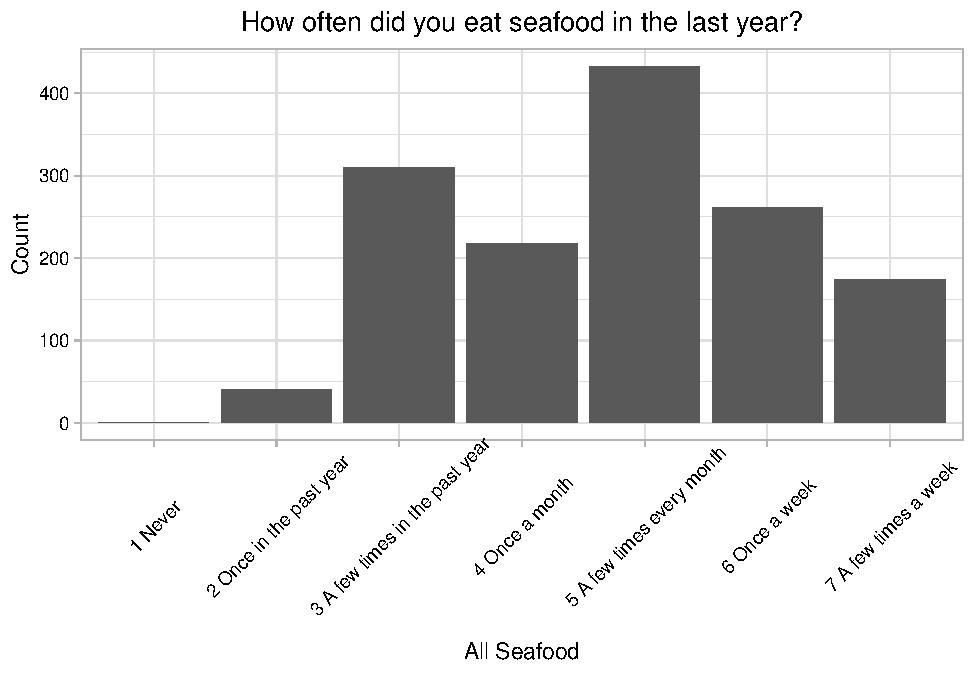
\includegraphics{Final_rmd_files/figure-latex/freq general-1.pdf}
freq.general mean = 4.76

\begin{itemize}
\tightlist
\item
  map of counties where respondents live?
\end{itemize}

\newpage

\hypertarget{analysis}{%
\section{Analysis}\label{analysis}}

\hypertarget{question-1a-when-consumers-buy-seafood-which-species-do-they-prefer}{%
\subsection{Question 1a: When consumers buy seafood, which species do
they
prefer?}\label{question-1a-when-consumers-buy-seafood-which-species-do-they-prefer}}

\begin{figure}
\centering
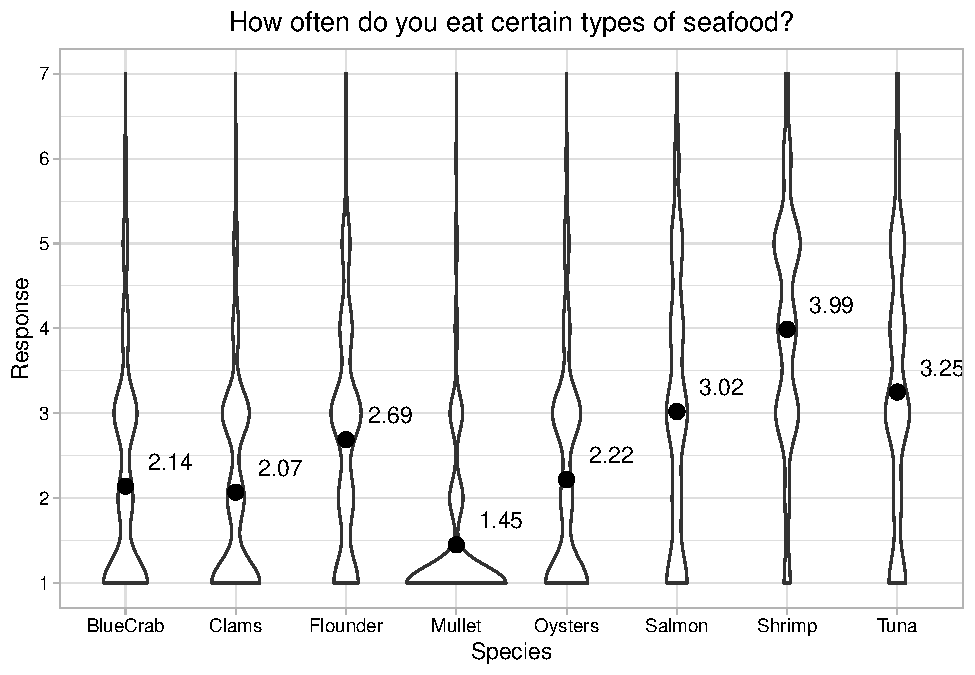
\includegraphics{Final_rmd_files/figure-latex/freq violin-1.pdf}
\caption{Violin plot and means of the frequency of seafood consumption
based on type}
\end{figure}

Based on this analysis, it appears as though respondents tended to eat
shrimp more than the other species and tended to eat mullet less than
the other species. However, the manner in which the chart conveys the
information masks some of the detail. With that in mind, we explore
other means of rendering the data.

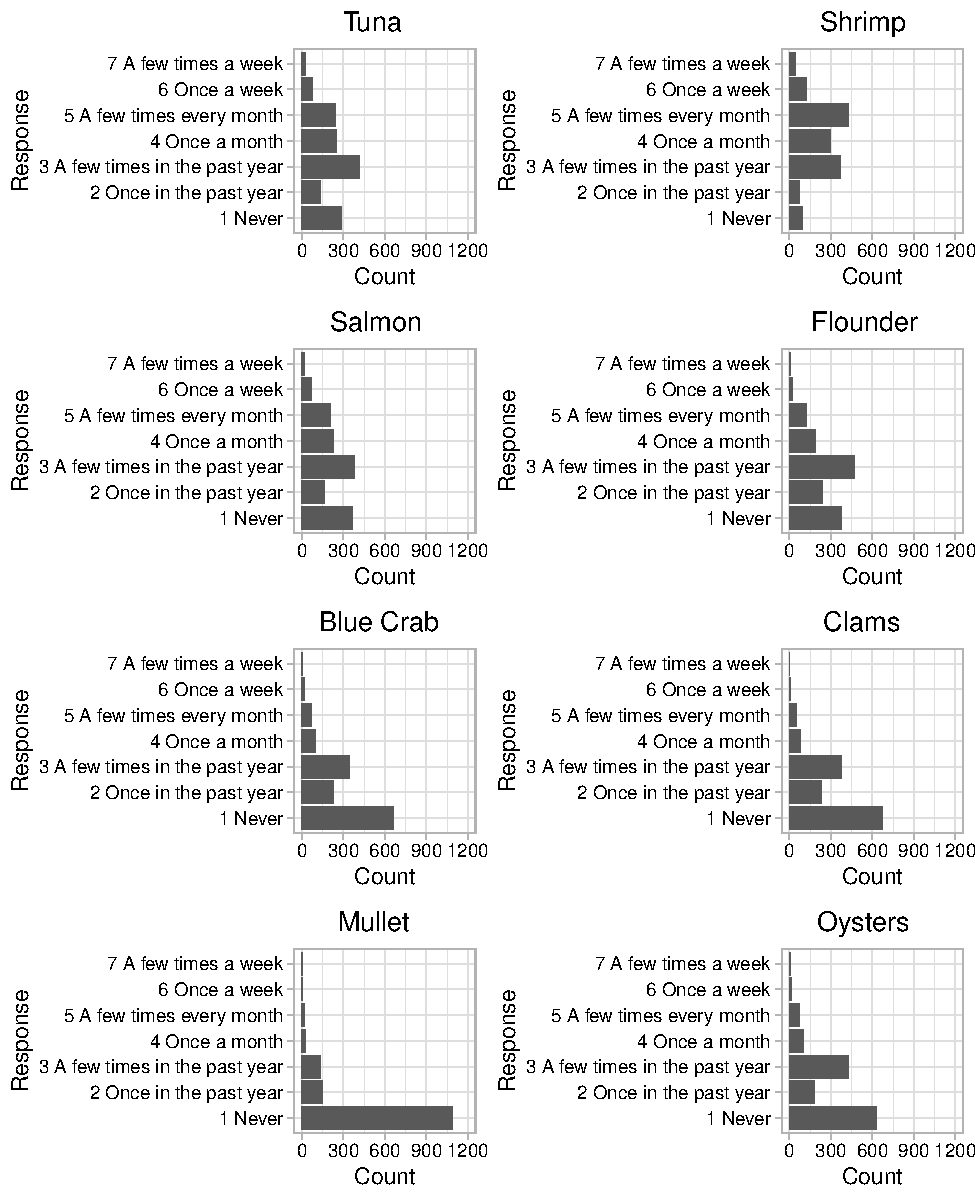
\includegraphics{Final_rmd_files/figure-latex/frequency-1.pdf} This
revised means of conveying the data does a much clearer job of showing
that respondents tend to eat Shrimp, Tuna, and Salmon more often than
they eat the other species. Respondents overwhelmingly never eat Mullet.
Respondents seem to eat Blue Crab, Clams, and Oysters very infrequently
if ever. However, this information is still pulled apart by frequency.
The below visualization simplifies the data even further, capturing the
number of respondents who ever consume each species.

{[}explanation etc{]}

\hypertarget{question-1b-do-consumers-prefer-wild-or-farmed-fish}{%
\subsubsection{Question 1b: Do consumers prefer wild or farmed
fish?}\label{question-1b-do-consumers-prefer-wild-or-farmed-fish}}

\begin{figure}
\centering
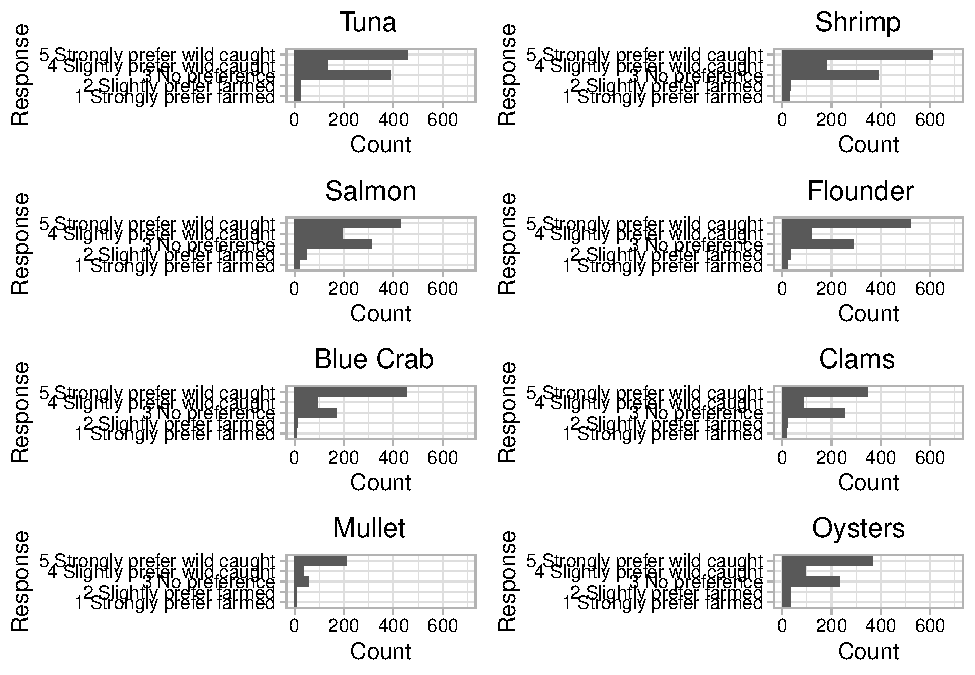
\includegraphics{Final_rmd_files/figure-latex/preference-1.pdf}
\caption{Do you prefer wild-caught or farmed versions of these seafood?}
\end{figure}

On the whole, respondents seem to have some degree of preference for
wild caught seafood or don't have any preference between wild caught and
farmed seafood. However, very few respondents identified any degree of
preference for farmed fish.

The species-specific barplots do a clear job of showing that the
preference trends remain relatively uniform across all species but with
a couple interesting points. For those species that respondents said
they consumed less often, Mullet and Blue Crab, respondents showed a
larger ``stronger preference for wild caught.'' Meanwhile, for those
species that respondents said they consumed more often, Tuna, Shrimp,
and Salmon, respondents identified ``no preference'' between farmed and
wild-caught a little more readily.

\hypertarget{question-2a-what-qualities-do-consumers-associate-with-seafood}{%
\subsection{Question 2a: What qualities do consumers associate with
seafood?}\label{question-2a-what-qualities-do-consumers-associate-with-seafood}}

\begin{figure}
\centering
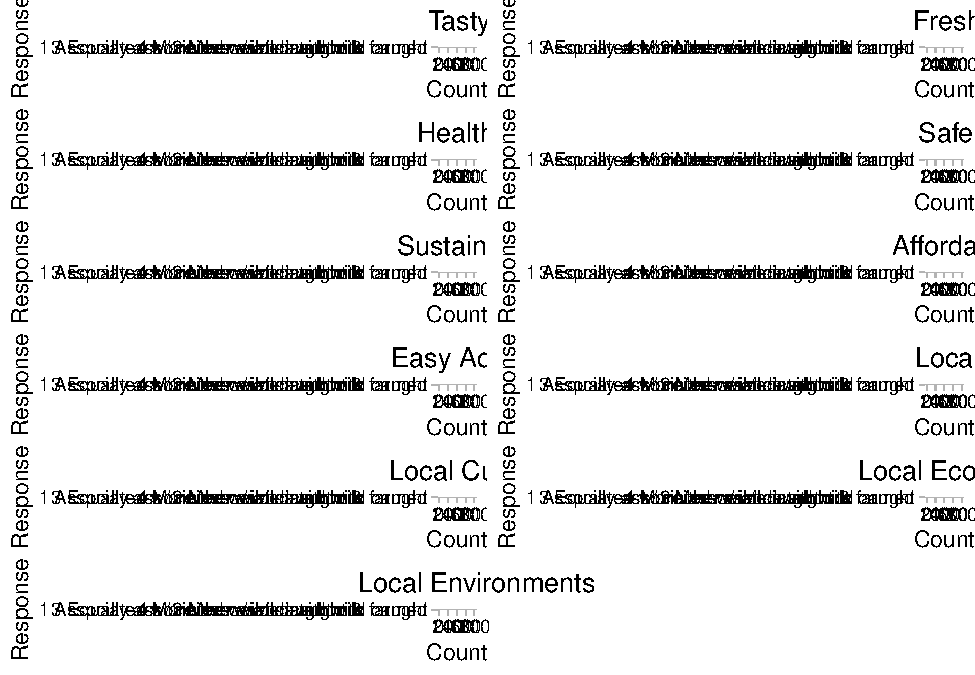
\includegraphics{Final_rmd_files/figure-latex/qualities-1.pdf}
\caption{How do you associate the following qualities with wild
vs.~farmed seafood?}
\end{figure}

There is quite the spread in associations of particular qualities with
farmed or wild-caught seafood. Given this spread and the challenges with
parsing apart the data in this format, we explore a different way of
visualizing data below.

This means of rendering the data shows that folks tend to associate
tasty, fresh, safe, healthy, and the various local categories more
heavily with wild-caught seafood. However, respondents tent to associate
sustainability, easy access, and affordability more heavily with farmed
seafood.

\hypertarget{question-2b-what-qualities-do-consumers-value-in-seafood}{%
\subsection{Question 2b: What qualities do consumers value in
seafood?}\label{question-2b-what-qualities-do-consumers-value-in-seafood}}

\begin{figure}
\centering
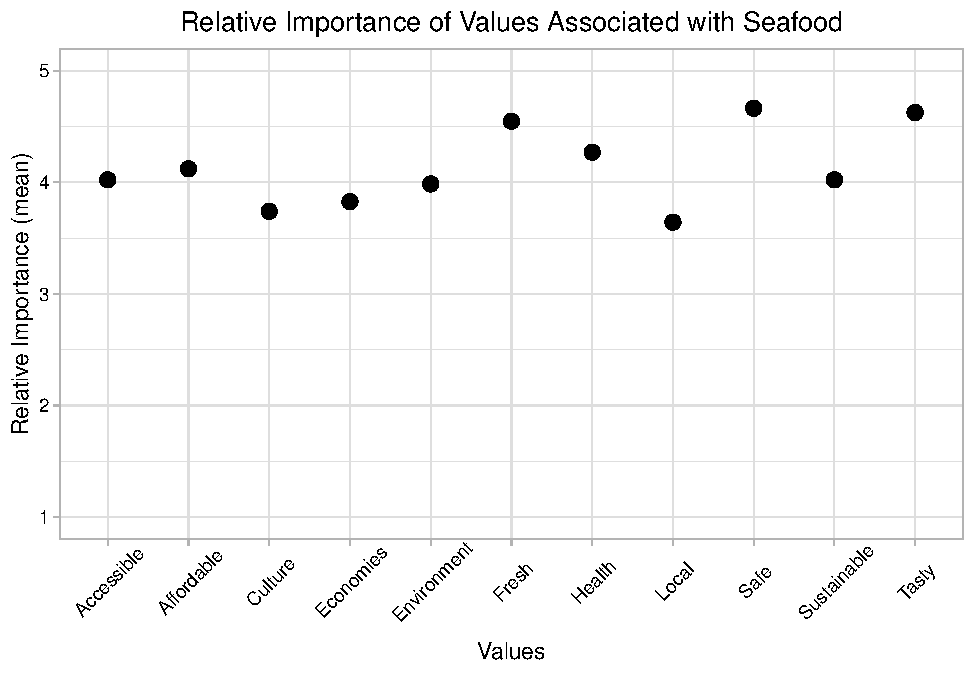
\includegraphics{Final_rmd_files/figure-latex/importance-1.pdf}
\caption{How important are the following qualities?}
\end{figure}

Here, we can see that respondents prioritized certain qualities like
safety, tastiness, freshness, and healthiness of the seafood but didn't
seem to place as much emphasis on other qualities like whether the
seafood was farmed or wild.

\hypertarget{question-3-are-valued-seafood-qualities-predicted-by-demographic-variables-such-as-age-or-education-level}{%
\subsection{Question 3: Are valued seafood qualities predicted by
demographic variables such as age or education
level?}\label{question-3-are-valued-seafood-qualities-predicted-by-demographic-variables-such-as-age-or-education-level}}

Fresh tasty healthy local - qualities most associated with wild

\begin{verbatim}
## 
## Call:
## lm(formula = Fresh ~ Age, data = demo.age)
## 
## Residuals:
##     Min      1Q  Median      3Q     Max 
## -3.6105 -0.5300  0.4151  0.4700  1.0000 
## 
## Coefficients:
##             Estimate Std. Error t value Pr(>|t|)    
## (Intercept)  4.00000    0.09923  40.311  < 2e-16 ***
## Age2         0.34826    0.11607   3.001  0.00276 ** 
## Age3         0.34118    0.11888   2.870  0.00419 ** 
## Age4         0.58491    0.12012   4.869 1.30e-06 ***
## Age5         0.55128    0.12049   4.575 5.33e-06 ***
## Age6         0.61047    0.11867   5.144 3.22e-07 ***
## Age7         0.53000    0.13089   4.049 5.53e-05 ***
## ---
## Signif. codes:  0 '***' 0.001 '**' 0.01 '*' 0.05 '.' 0.1 ' ' 1
## 
## Residual standard error: 0.8536 on 1025 degrees of freedom
## Multiple R-squared:  0.03693,    Adjusted R-squared:  0.0313 
## F-statistic: 6.551 on 6 and 1025 DF,  p-value: 8.386e-07
\end{verbatim}

\begin{verbatim}
## 
## Call:
## lm(formula = Fresh ~ Education, data = demo.ed)
## 
## Residuals:
##     Min      1Q  Median      3Q     Max 
## -3.6808 -0.5331  0.4215  0.4669  0.9143 
## 
## Coefficients:
##             Estimate Std. Error t value Pr(>|t|)    
## (Intercept)   4.0857     0.1330  30.730  < 2e-16 ***
## Education2    0.3029     0.1428   2.122 0.034006 *  
## Education3    0.4474     0.1404   3.186 0.001477 ** 
## Education4    0.4772     0.1462   3.263 0.001128 ** 
## Education5    0.4928     0.1389   3.548 0.000401 ***
## Education6    0.5951     0.1416   4.202 2.81e-05 ***
## Education7    0.5265     0.1741   3.025 0.002534 ** 
## ---
## Signif. codes:  0 '***' 0.001 '**' 0.01 '*' 0.05 '.' 0.1 ' ' 1
## 
## Residual standard error: 0.7866 on 1417 degrees of freedom
## Multiple R-squared:  0.02069,    Adjusted R-squared:  0.01654 
## F-statistic: 4.989 on 6 and 1417 DF,  p-value: 4.553e-05
\end{verbatim}

\begin{verbatim}
## 
## Call:
## lm(formula = Fresh ~ Political_Party, data = demo.party)
## 
## Residuals:
##     Min      1Q  Median      3Q     Max 
## -3.6125 -0.5730  0.3875  0.4270  0.4270 
## 
## Coefficients:
##                  Estimate Std. Error t value Pr(>|t|)    
## (Intercept)       4.61247    0.03488 132.243   <2e-16 ***
## Political_Party2 -0.03949    0.04906  -0.805    0.421    
## ---
## Signif. codes:  0 '***' 0.001 '**' 0.01 '*' 0.05 '.' 0.1 ' ' 1
## 
## Residual standard error: 0.7391 on 906 degrees of freedom
## Multiple R-squared:  0.0007146,  Adjusted R-squared:  -0.0003883 
## F-statistic: 0.6479 on 1 and 906 DF,  p-value: 0.4211
\end{verbatim}

\begin{verbatim}
## 
## Call:
## lm(formula = Local ~ Age, data = demo.age)
## 
## Residuals:
##     Min      1Q  Median      3Q     Max 
## -2.6164 -0.6163 -0.2289  0.7711  1.8649 
## 
## Coefficients:
##             Estimate Std. Error t value Pr(>|t|)    
## (Intercept)  3.13514    0.14044  22.324  < 2e-16 ***
## Age2         0.09372    0.16427   0.571  0.56845    
## Age3         0.12957    0.16825   0.770  0.44142    
## Age4         0.48122    0.17001   2.831  0.00474 ** 
## Age5         0.37769    0.17053   2.215  0.02699 *  
## Age6         0.37068    0.16796   2.207  0.02753 *  
## Age7         0.12486    0.18525   0.674  0.50045    
## ---
## Signif. codes:  0 '***' 0.001 '**' 0.01 '*' 0.05 '.' 0.1 ' ' 1
## 
## Residual standard error: 1.208 on 1025 degrees of freedom
## Multiple R-squared:  0.01778,    Adjusted R-squared:  0.01203 
## F-statistic: 3.093 on 6 and 1025 DF,  p-value: 0.005248
\end{verbatim}

\begin{verbatim}
## 
## Call:
## lm(formula = Local ~ Education, data = demo.ed)
## 
## Residuals:
##     Min      1Q  Median      3Q     Max 
## -2.8846 -0.6911  0.3089  1.1154  1.5714 
## 
## Coefficients:
##             Estimate Std. Error t value Pr(>|t|)    
## (Intercept)  3.42857    0.20118  17.042   <2e-16 ***
## Education2   0.07361    0.21601   0.341   0.7333    
## Education3   0.11447    0.21252   0.539   0.5902    
## Education4   0.08041    0.22126   0.363   0.7163    
## Education5   0.26253    0.21019   1.249   0.2119    
## Education6   0.45604    0.21429   2.128   0.0335 *  
## Education7   0.40816    0.26341   1.550   0.1215    
## ---
## Signif. codes:  0 '***' 0.001 '**' 0.01 '*' 0.05 '.' 0.1 ' ' 1
## 
## Residual standard error: 1.19 on 1417 degrees of freedom
## Multiple R-squared:  0.01476,    Adjusted R-squared:  0.01059 
## F-statistic: 3.537 on 6 and 1417 DF,  p-value: 0.001762
\end{verbatim}

\begin{verbatim}
## 
## Call:
## lm(formula = Local ~ Political_Party, data = demo.party)
## 
## Residuals:
##     Min      1Q  Median      3Q     Max 
## -2.7734 -0.7734  0.2266  1.2266  1.3185 
## 
## Coefficients:
##                  Estimate Std. Error t value Pr(>|t|)    
## (Intercept)       3.68151    0.05561  66.205   <2e-16 ***
## Political_Party2  0.09191    0.07821   1.175     0.24    
## ---
## Signif. codes:  0 '***' 0.001 '**' 0.01 '*' 0.05 '.' 0.1 ' ' 1
## 
## Residual standard error: 1.178 on 906 degrees of freedom
## Multiple R-squared:  0.001522,   Adjusted R-squared:  0.0004197 
## F-statistic: 1.381 on 1 and 906 DF,  p-value: 0.2403
\end{verbatim}

\begin{verbatim}
## 
## Call:
## lm(formula = Tasty ~ Age, data = demo.age)
## 
## Residuals:
##     Min      1Q  Median      3Q     Max 
## -3.6667 -0.4677  0.3430  0.4647  0.5676 
## 
## Coefficients:
##             Estimate Std. Error t value Pr(>|t|)    
## (Intercept)  4.43243    0.08570  51.722   <2e-16 ***
## Age2         0.03523    0.10024   0.351   0.7253    
## Age3         0.10286    0.10267   1.002   0.3166    
## Age4         0.19021    0.10374   1.834   0.0670 .  
## Age5         0.23423    0.10406   2.251   0.0246 *  
## Age6         0.22454    0.10249   2.191   0.0287 *  
## Age7         0.24757    0.11304   2.190   0.0287 *  
## ---
## Signif. codes:  0 '***' 0.001 '**' 0.01 '*' 0.05 '.' 0.1 ' ' 1
## 
## Residual standard error: 0.7372 on 1025 degrees of freedom
## Multiple R-squared:  0.01409,    Adjusted R-squared:  0.008321 
## F-statistic: 2.442 on 6 and 1025 DF,  p-value: 0.02383
\end{verbatim}

\begin{verbatim}
## 
## Call:
## lm(formula = Tasty ~ Education, data = demo.ed)
## 
## Residuals:
##     Min      1Q  Median      3Q     Max 
## -3.6615 -0.6122  0.3403  0.3444  0.7143 
## 
## Coefficients:
##             Estimate Std. Error t value Pr(>|t|)    
## (Intercept)   4.2857     0.1145  37.426  < 2e-16 ***
## Education2    0.2645     0.1230   2.151  0.03162 *  
## Education3    0.3699     0.1210   3.058  0.00227 ** 
## Education4    0.3490     0.1259   2.771  0.00566 ** 
## Education5    0.3740     0.1196   3.126  0.00181 ** 
## Education6    0.3758     0.1220   3.081  0.00210 ** 
## Education7    0.3265     0.1499   2.178  0.02958 *  
## ---
## Signif. codes:  0 '***' 0.001 '**' 0.01 '*' 0.05 '.' 0.1 ' ' 1
## 
## Residual standard error: 0.6775 on 1417 degrees of freedom
## Multiple R-squared:  0.009764,   Adjusted R-squared:  0.005571 
## F-statistic: 2.329 on 6 and 1417 DF,  p-value: 0.03051
\end{verbatim}

\begin{verbatim}
## 
## Call:
## lm(formula = Tasty ~ Political_Party, data = demo.party)
## 
## Residuals:
##     Min      1Q  Median      3Q     Max 
## -3.6904 -0.6275  0.3096  0.3725  0.3725 
## 
## Coefficients:
##                  Estimate Std. Error t value Pr(>|t|)    
## (Intercept)       4.69042    0.02980 157.394   <2e-16 ***
## Political_Party2 -0.06297    0.04191  -1.502    0.133    
## ---
## Signif. codes:  0 '***' 0.001 '**' 0.01 '*' 0.05 '.' 0.1 ' ' 1
## 
## Residual standard error: 0.6315 on 906 degrees of freedom
## Multiple R-squared:  0.002485,   Adjusted R-squared:  0.001384 
## F-statistic: 2.257 on 1 and 906 DF,  p-value: 0.1333
\end{verbatim}

\begin{verbatim}
## 
## Call:
## lm(formula = Health ~ Age, data = demo.age)
## 
## Residuals:
##     Min      1Q  Median      3Q     Max 
## -3.3372 -0.3372 -0.0882  0.7610  0.9865 
## 
## Coefficients:
##             Estimate Std. Error t value Pr(>|t|)    
## (Intercept)  4.01351    0.11050  36.321   <2e-16 ***
## Age2         0.14569    0.12925   1.127   0.2599    
## Age3         0.07472    0.13239   0.564   0.5726    
## Age4         0.22548    0.13377   1.686   0.0922 .  
## Age5         0.27495    0.13418   2.049   0.0407 *  
## Age6         0.32370    0.13215   2.449   0.0145 *  
## Age7         0.24649    0.14576   1.691   0.0911 .  
## ---
## Signif. codes:  0 '***' 0.001 '**' 0.01 '*' 0.05 '.' 0.1 ' ' 1
## 
## Residual standard error: 0.9506 on 1025 degrees of freedom
## Multiple R-squared:  0.0107, Adjusted R-squared:  0.004912 
## F-statistic: 1.848 on 6 and 1025 DF,  p-value: 0.0868
\end{verbatim}

\begin{verbatim}
## 
## Call:
## lm(formula = Health ~ Education, data = demo.ed)
## 
## Residuals:
##     Min      1Q  Median      3Q     Max 
## -3.3500 -0.3477  0.6500  0.7120  1.2000 
## 
## Coefficients:
##             Estimate Std. Error t value Pr(>|t|)    
## (Intercept)   3.8000     0.1537  24.723  < 2e-16 ***
## Education2    0.3528     0.1650   2.138 0.032685 *  
## Education3    0.5477     0.1624   3.373 0.000763 ***
## Education4    0.4335     0.1690   2.565 0.010431 *  
## Education5    0.4880     0.1606   3.039 0.002421 ** 
## Education6    0.5500     0.1637   3.359 0.000802 ***
## Education7    0.4245     0.2012   2.109 0.035090 *  
## ---
## Signif. codes:  0 '***' 0.001 '**' 0.01 '*' 0.05 '.' 0.1 ' ' 1
## 
## Residual standard error: 0.9093 on 1417 degrees of freedom
## Multiple R-squared:  0.01248,    Adjusted R-squared:  0.008299 
## F-statistic: 2.985 on 6 and 1417 DF,  p-value: 0.006693
\end{verbatim}

\begin{verbatim}
## 
## Call:
## lm(formula = Health ~ Political_Party, data = demo.party)
## 
## Residuals:
##     Min      1Q  Median      3Q     Max 
## -3.3486 -0.3486  0.6514  0.6514  0.6882 
## 
## Coefficients:
##                  Estimate Std. Error t value Pr(>|t|)    
## (Intercept)       4.31180    0.03962  108.83   <2e-16 ***
## Political_Party2  0.03678    0.05573    0.66    0.509    
## ---
## Signif. codes:  0 '***' 0.001 '**' 0.01 '*' 0.05 '.' 0.1 ' ' 1
## 
## Residual standard error: 0.8395 on 906 degrees of freedom
## Multiple R-squared:  0.0004806,  Adjusted R-squared:  -0.0006226 
## F-statistic: 0.4356 on 1 and 906 DF,  p-value: 0.5094
\end{verbatim}

\newpage

\hypertarget{summary-and-conclusions}{%
\section{Summary and Conclusions}\label{summary-and-conclusions}}

\newpage

\hypertarget{references}{%
\section{References}\label{references}}

\textless add references here if relevant, otherwise delete this
section\textgreater{}

\end{document}
